\documentclass[italian,a4paper, twoside, 12pt]{report}
\usepackage{lmodern}
\usepackage{amssymb,amsmath}
\usepackage{ifxetex,ifluatex}
\usepackage{fixltx2e} % provides \textsubscript
\ifnum 0\ifxetex 1\fi\ifluatex 1\fi=0 % if pdftex
  \usepackage[T1]{fontenc}
  \usepackage[utf8]{inputenc}
\else % if luatex or xelatex
  \ifxetex
    \usepackage{mathspec}
  \else
    \usepackage{fontspec}
  \fi
  \defaultfontfeatures{Ligatures=TeX,Scale=MatchLowercase}
    \setmainfont[]{Palatino Linotype}
    \setmonofont[Mapping=tex-ansi]{InconsolataForPowerline Nerd Font}
\fi
% use upquote if available, for straight quotes in verbatim environments
\IfFileExists{upquote.sty}{\usepackage{upquote}}{}
% use microtype if available
\IfFileExists{microtype.sty}{%
\usepackage[]{microtype}
\UseMicrotypeSet[protrusion]{basicmath} % disable protrusion for tt fonts
}{}
\PassOptionsToPackage{hyphens}{url} % url is loaded by hyperref
\usepackage[unicode=true]{hyperref}
\PassOptionsToPackage{usenames,dvipsnames}{color} % color is loaded by hyperref
\hypersetup{
            colorlinks=true,
            linkcolor=Maroon,
            citecolor=Blue,
            urlcolor=NavyBlue,
            breaklinks=true}
\urlstyle{same}  % don't use monospace font for urls
\usepackage[a4paper, left=3.5cm, right=3cm, top=2.5cm, bottom=3cm]{geometry}
\ifnum 0\ifxetex 1\fi\ifluatex 1\fi=0 % if pdftex
  \usepackage[shorthands=off,main=italian]{babel}
\else
  \usepackage{polyglossia}
  \setmainlanguage[]{italian}
\fi
\usepackage{color}
\usepackage{fancyvrb}
\newcommand{\VerbBar}{|}
\newcommand{\VERB}{\Verb[commandchars=\\\{\}]}
\DefineVerbatimEnvironment{Highlighting}{Verbatim}{commandchars=\\\{\}}
% Add ',fontsize=\small' for more characters per line
\newenvironment{Shaded}{}{}
\newcommand{\KeywordTok}[1]{\textcolor[rgb]{0.00,0.44,0.13}{\textbf{#1}}}
\newcommand{\DataTypeTok}[1]{\textcolor[rgb]{0.56,0.13,0.00}{#1}}
\newcommand{\DecValTok}[1]{\textcolor[rgb]{0.25,0.63,0.44}{#1}}
\newcommand{\BaseNTok}[1]{\textcolor[rgb]{0.25,0.63,0.44}{#1}}
\newcommand{\FloatTok}[1]{\textcolor[rgb]{0.25,0.63,0.44}{#1}}
\newcommand{\ConstantTok}[1]{\textcolor[rgb]{0.53,0.00,0.00}{#1}}
\newcommand{\CharTok}[1]{\textcolor[rgb]{0.25,0.44,0.63}{#1}}
\newcommand{\SpecialCharTok}[1]{\textcolor[rgb]{0.25,0.44,0.63}{#1}}
\newcommand{\StringTok}[1]{\textcolor[rgb]{0.25,0.44,0.63}{#1}}
\newcommand{\VerbatimStringTok}[1]{\textcolor[rgb]{0.25,0.44,0.63}{#1}}
\newcommand{\SpecialStringTok}[1]{\textcolor[rgb]{0.73,0.40,0.53}{#1}}
\newcommand{\ImportTok}[1]{#1}
\newcommand{\CommentTok}[1]{\textcolor[rgb]{0.38,0.63,0.69}{\textit{#1}}}
\newcommand{\DocumentationTok}[1]{\textcolor[rgb]{0.73,0.13,0.13}{\textit{#1}}}
\newcommand{\AnnotationTok}[1]{\textcolor[rgb]{0.38,0.63,0.69}{\textbf{\textit{#1}}}}
\newcommand{\CommentVarTok}[1]{\textcolor[rgb]{0.38,0.63,0.69}{\textbf{\textit{#1}}}}
\newcommand{\OtherTok}[1]{\textcolor[rgb]{0.00,0.44,0.13}{#1}}
\newcommand{\FunctionTok}[1]{\textcolor[rgb]{0.02,0.16,0.49}{#1}}
\newcommand{\VariableTok}[1]{\textcolor[rgb]{0.10,0.09,0.49}{#1}}
\newcommand{\ControlFlowTok}[1]{\textcolor[rgb]{0.00,0.44,0.13}{\textbf{#1}}}
\newcommand{\OperatorTok}[1]{\textcolor[rgb]{0.40,0.40,0.40}{#1}}
\newcommand{\BuiltInTok}[1]{#1}
\newcommand{\ExtensionTok}[1]{#1}
\newcommand{\PreprocessorTok}[1]{\textcolor[rgb]{0.74,0.48,0.00}{#1}}
\newcommand{\AttributeTok}[1]{\textcolor[rgb]{0.49,0.56,0.16}{#1}}
\newcommand{\RegionMarkerTok}[1]{#1}
\newcommand{\InformationTok}[1]{\textcolor[rgb]{0.38,0.63,0.69}{\textbf{\textit{#1}}}}
\newcommand{\WarningTok}[1]{\textcolor[rgb]{0.38,0.63,0.69}{\textbf{\textit{#1}}}}
\newcommand{\AlertTok}[1]{\textcolor[rgb]{1.00,0.00,0.00}{\textbf{#1}}}
\newcommand{\ErrorTok}[1]{\textcolor[rgb]{1.00,0.00,0.00}{\textbf{#1}}}
\newcommand{\NormalTok}[1]{#1}
\usepackage{longtable,booktabs}
% Fix footnotes in tables (requires footnote package)
\IfFileExists{footnote.sty}{\usepackage{footnote}\makesavenoteenv{long table}}{}
\usepackage{graphicx,grffile}
\makeatletter
\def\maxwidth{\ifdim\Gin@nat@width>\linewidth\linewidth\else\Gin@nat@width\fi}
\def\maxheight{\ifdim\Gin@nat@height>\textheight\textheight\else\Gin@nat@height\fi}
\makeatother
% Scale images if necessary, so that they will not overflow the page
% margins by default, and it is still possible to overwrite the defaults
% using explicit options in \includegraphics[width, height, ...]{}
\setkeys{Gin}{width=\maxwidth,height=\maxheight,keepaspectratio}
\IfFileExists{parskip.sty}{%
\usepackage{parskip}
}{% else
\setlength{\parindent}{0pt}
\setlength{\parskip}{6pt plus 2pt minus 1pt}
}
\setlength{\emergencystretch}{3em}  % prevent overfull lines
\providecommand{\tightlist}{%
  \setlength{\itemsep}{0pt}\setlength{\parskip}{0pt}}
\setcounter{secnumdepth}{0}
% Redefines (sub)paragraphs to behave more like sections
\ifx\paragraph\undefined\else
\let\oldparagraph\paragraph
\renewcommand{\paragraph}[1]{\oldparagraph{#1}\mbox{}}
\fi
\ifx\subparagraph\undefined\else
\let\oldsubparagraph\subparagraph
\renewcommand{\subparagraph}[1]{\oldsubparagraph{#1}\mbox{}}
\fi

% set default figure placement to htbp
\makeatletter
\def\fps@figure{htbp}
\makeatother

\usepackage[dvipsnames]{xcolor}
\usepackage{tikz}
\usetikzlibrary{calc}
\addto\captionsitalian{\renewcommand{\chaptername}{Parte}}
\renewcommand{\baselinestretch}{1.1} 
% \renewcommand\thechapter{\Roman{chapter}}

% set default figure placement to htbp
\makeatletter
\def\fps@figure{htbp}
\makeatother

\usepackage{subfig}
\usepackage{float}
\floatstyle{plain}
\makeatletter
\@ifundefined{c@chapter}{\newfloat{codelisting}{h}{lop}}{\newfloat{codelisting}{h}{lop}[chapter]}
\makeatother
\floatname{codelisting}{Listato}
\newcommand*\listoflistings{\listof{codelisting}{Elenco dei Listati}}

\date{}

\begin{document}

\definecolor{unicamblue}{HTML}{002860}

\newgeometry{left=2.25cm,right=2.25cm,top=1cm,bottom=1cm,a4paper}

\begin{titlepage}
    \color{unicamblue}

\begin{tikzpicture}[remember picture, overlay]
    \color{black}
  \draw[line width = 0.5pt] ($(current page.north west) + (1cm,-1cm)$) rectangle ($(current page.south east) + (-1cm,1cm)$);
\end{tikzpicture}

\begin{center}

\vspace{1cm}
\Huge\sc Università degli Studi di Camerino\\
\vspace{3mm}
\huge\bf Scuola di Scienze e Tecnologie\\
\vspace{3mm}
    \LARGE \bf \textsl{Corso di Laurea in Informatica}
\end{center}

\vspace{14mm}

\begin{center}


\includegraphics[width=3.5cm]{img/unicam_logo.pdf}\\

\vspace{1.5cm}
{\Huge{\bf Big Data}}\\
\vspace{5mm}
{\huge{\bf Tecniche e tool di analisi}}\\
\vspace{15mm} {\huge{Elaborato Finale}}

\end{center}

\vspace{25mm}
\par
\noindent

\begin{minipage}[t]{0.47\textwidth}
    \begin{center}
    {\LARGE{\textsl{Laureando}
    \vspace{0.2cm}\\
    \textbf{Emanuele Gentiletti}\\
    \vspace{1.7cm}
    Matricola: \textbf{090150}
    }}

    \end{center}
\end{minipage}
\hfill
\begin{minipage}[t]{0.47\textwidth}
    \begin{center}
    {\LARGE{\textsl{Relatore}
    \vspace{0.2cm}\\
    \bf Prof. Diletta Romana Cacciagrano\\
    }}

    \end{center}
\end{minipage}
\vspace{35mm}
\begin{center}
\rule[0.1cm]{14cm}{0.1mm}\\
\vspace{2mm}
{\Large{\textsl{Anno Accademico 2016/2017}}}
\end{center}
\end{titlepage}
\restoregeometry
\clearpage
\cleardoublepage

{
\hypersetup{linkcolor=black}
\setcounter{tocdepth}{2}
\tableofcontents
}
\clearpage

\chapter*{Introduzione}\label{introduzione}
\addcontentsline{toc}{chapter}{Introduzione}

Negli ultimi decenni, i Big Data hanno preso piede in modo impetuoso in
una grande varietà di ambiti. Il fenomeno ha avuto un enorme impatto:
settori come medicina, finanza, business analytics e marketing sfruttano
i Big Data per guidare lo sviluppo in modi semplicemente non possibili
prima.

L'innovazione che rende possibili questi risultati è guidata dal
software molto più che dall'hardware. Ci sono stati dei grandi
cambiamenti nel modo di pensare alla computazione e all'organizzazione
dei suoi processi, che hanno portato a risultati notevoli
nell'efficienza di elaborazione di grandi quantità di dati.

Uno dei più importanti fenomeni che hanno portato a questa spinta è
stato lo sviluppo di Hadoop, un framework open source progettato per la
computazione batch di dataset di grandi dimensioni. Utilizzando
un'architettura ben congeniata, Hadoop ha permesso l'analisi in tempi
molto rapidi di interi dataset di dimensioni nell'ordine dei terabyte,
fornendo una capacità di sfruttamento di questi, e conseguentemente un
valore molto più alti.

Una delle conseguenze più importanti di Hadoop è stata una
democratizzazione delle capacità di analisi dei dati:

\begin{itemize}
\tightlist
\item
  Hadoop è sotto licenza Apache, permettendo a chiunque di utilizzarlo a
  scopi commerciali e non;
\item
  Hadoop non richiede hardware costoso ad alta affidabilità, e
  incoraggia l'adozione di macchine più generiche e prone al fallimento
  per il suo uso, che possono essere ottenute a costi inferiori;
\item
  Il design di Hadoop permette la sua esecuzione in cluster di macchine
  eterogenee nel software e nell'hardware che possono essere acquisite
  da diversi rivenditori, un altro fattore che permette l'abbattimento
  dei costi;
\item
  I vari modelli di programmazione in Hadoop hanno in comune
  l'astrazione della computazione distribuita e dei problemi intricati
  che questa comporta, abbassando la barriere in entrata in termini di
  conoscenze e lavoro richiesti per creare programmi che necessitano di
  un altro grado di parallelismo.
\end{itemize}

Questi fattori hanno spinto a una vasta adozione di Hadoop e
dell'ecosistema software che lo circonda, in ambito aziendale e
scientifico. L'adozione di Hadoop, secondo un sondaggio fatto a maggio
2015{[}\protect\hyperlink{ref-hadoop-adoption-survey}{2}{]}, si aggira
al 26\% delle imprese negli Stati Uniti, e si prevede che il mercato
attorno ad Hadoop sorpasserà i 16 miliardi di dollari nel 2020
{[}\protect\hyperlink{ref-hadoop-market-analysis}{3}{]}.

Tutto questo accade in un'ottica in cui la produzione di informazioni
aumenta ad una scala senza precedenti: secondo uno studio di
IDC{[}\protect\hyperlink{ref-digital-univ}{4}{]}, la quantità di
informazioni nell'``Universo Digitale'' ammontava a 4.4 TB nel 2014, e
la sua dimensione stimata nel 2020 è di 44 TB.

Data la presenza di questa vasta quantità di informazioni, lo
sfruttamento efficace di queste è fonte di grandi opportunità. In questo
documento si analizzano le varie tecniche che sono a disposizione per
l'utilizzo effettivo dei Big Data, come queste differiscono tra di loro,
e quali strumenti le mettono a disposizione. Si parlerà inoltre di come
gli strumenti possano essere integrati in sistemi di produzione
esistenti, le possibili architetture di un sistema di questo tipo e come
\ldots{}

La gestione di sistemi per l'elaborazione di Big Data richiede una
configurazione accurata per ottenere affidabilità e fault-tolerance. Pur
sottolineando che l'importanza di questi aspetti non è da sottovalutare,
questa tesi si concentrerà più sul modello computazionale e di
programmazione che gli strumenti offrono.

\chapter{Big Data e Paradigmi di
Elaborazione}\label{big-data-e-paradigmi-di-elaborazione}

Per Big Data si intendono collezioni di dati con caratteristiche tali da
richiedere strumenti innovativi per poterli gestire e analizzare. Uno
dei modelli tradizionali e più popolari per descrivere le
caratteristiche dei Big Data si chiama \textbf{modello delle 3V}. Il
modello identifica i Big Data come collezioni di informazione che
presentano grande abbondanza in una più delle seguenti caratteristiche:

\begin{itemize}
\tightlist
\item
  Il \textbf{volume} delle informazioni, che può aggirarsi dalle decine
  di terabyte per arrivare all'ordine dei petabyte;
\item
  La \textbf{varietà}, intesa come la varietà di \emph{fonti} e di
  \emph{possibili strutturazioni} delle informazioni di interesse;
\item
  La \textbf{velocità} di produzione delle informazioni di interesse.
\end{itemize}

Ognuno dei punti di questo modello deriva da esigenze che vanno ad
accentuarsi andando avanti nel tempo, in particolare:

\begin{itemize}
\item
  Il volume delle collezioni dei dati è aumentato esponenzialmente in
  tempi recenti, con l'avvento dei Social Media, dell'IOT, e degli
  smartphone muniti di molti sensori diversi. Generalizzando, i fattori
  che hanno portato a un grande incremento del volume dei data set sono
  un aumento della generazione automatica di dati da parte dei
  dispositivi e dei contenuti prodotti dagli utenti.
\item
  L'aumento dei dispositivi e dei dati generati dagli utenti portano
  conseguentemente a un aumento delle fonti dei dati, ed essendo queste
  gestite da enti e persone diverse la struttura che le fonti presentano
  difficilmente sarà uniforme, l'una rispetto all'altra. Inoltre,
  l'utilizzo di dati non strutturati rigidamente è prevalente nelle
  tecnologie web (in particolare documenti JSON), che sono spesso un
  obiettivo desiderabile di analisi.
\item
  Si possono fare le stesse considerazioni fatte per il volume dei dati
  per quanto riguarda la velocità. I flussi di dati vengono generati dai
  dispositivi e dagli utenti, che li producono a velocità molto maggiori
  rispetto agli operatori.
\end{itemize}

Per l'elaborazione di dataset con queste caratteristiche sono stati
sviluppati molti strumenti, che usano diversi pattern di elaborazione a
seconda delle esigenze dell'utente e del tipo di dati con cui si ha a
che fare. I modelli di elaborazione più importanti e rappresentativi
sono il \emph{batch processing} e lo \emph{stream processing}.

\section{Batch e Streaming
Processing}\label{batch-e-streaming-processing}

Il batch processing è il pattern di elaborazione generalmente più
efficiente, e consiste nell'elaborazione di un intero dataset in
un'unità di lavoro, per poi ottenere i risultati al termine di questa.

Questo approccio è ottimale quando non c'è una necessità impendente di
avere risultati, ma in alcuni casi è necessario avere i risultati a
disposizione mano a mano che la computazione procede, e il batch
processing non è adatto a questo scopo:

\begin{itemize}
\item
  Le fasi del batch processing richiedono la schedulazione dei lavori da
  parte dell'utente, con un conseguente overhead dovuto alla
  schedulazione in sé o alla configurazione di strumenti automatizzati
  che se ne occupino;
\item
  Non è possibile accedere ai risultati prima del termine del job, che
  può avere una durata eccessiva rispetto alle esigenze
  dell'applicazione o dell'utente.
\end{itemize}

Per use case in cui questi fattori sono rilevanti, lo \textbf{stream
processing} si presta come più adatto. In questo paradigma, i dati da
elaborare vengono ricevuti da stream (nella maggior parte dei casi da
Internet) e vengono processati mano a mano con il loro arrivo. I job in
streaming molto spesso non hanno un termine prestabilito, ma vengono
terminati dall'utente, e i risultati dell'elaborazione possono essere
disponibili mano a mano che l'elaborazione procede, permettendo quindi
un feedback più rapido rispetto ai lavori batch.

\subsection{\texorpdfstring{\emph{Data at Rest} e \emph{Data in
Motion}}{Data at Rest e Data in Motion}}\label{data-at-rest-e-data-in-motion}

I due paradigmi si differenziano anche per il modo in cui i dati sono
disponibili. Il processing batch richiede che l'informazione sia
\emph{data at rest}, ovvero informazioni salvate interamente in un mezzo
di memoria accessibile al programma. I dati di input in una computazione
batch sono determinati all'inizio dell'elaborazione, e non possono
cambiare nel corso di questa. Questo significa che se nuova informazione
arriva nel corso di un job batch, questa non può essere tenuta in conto
nell'elaborazione finale.

Lo \textbf{stream processing}, invece, è progettato per \emph{data in
motion}, dati in arrivo continuo la cui quantità non è fissa a priori. È
possibile utilizzare strumenti di processing in streaming anche per
\emph{data at rest}, rappresentando il dataset come uno stream. Questa
proprietà è desiderabile, perché permette di utilizzare le stesse
applicazioni per l'elaborazione di dati in arrivo dalla rete e quelli
salvati. Come si vedrà, la Kappa architecture, ovvero una possibile
architettura software per l'elaborazione di Big Data, utilizza questa
proprietà per sfruttare un solo paradigma sia per computazioni in
real-time di dati in arrivo da stream, che per i dati salvati
storicamente, permettendo di utilizzare gli stessi tool e interfacce di
programmazione per entrambi i tipi di elaborazione e massimizzare il
riutilizzo di codice.

\begin{longtable}[]{@{}lll@{}}
\caption{Differenze tra elaborazione batch e streaming}\tabularnewline
\toprule
\begin{minipage}[b]{0.27\columnwidth}\raggedright\strut
Caratteristiche\strut
\end{minipage} & \begin{minipage}[b]{0.21\columnwidth}\raggedright\strut
Batch\strut
\end{minipage} & \begin{minipage}[b]{0.43\columnwidth}\raggedright\strut
Streaming\strut
\end{minipage}\tabularnewline
\midrule
\endfirsthead
\toprule
\begin{minipage}[b]{0.27\columnwidth}\raggedright\strut
Caratteristiche\strut
\end{minipage} & \begin{minipage}[b]{0.21\columnwidth}\raggedright\strut
Batch\strut
\end{minipage} & \begin{minipage}[b]{0.43\columnwidth}\raggedright\strut
Streaming\strut
\end{minipage}\tabularnewline
\midrule
\endhead
\begin{minipage}[t]{0.27\columnwidth}\raggedright\strut
Ottimizzazione\strut
\end{minipage} & \begin{minipage}[t]{0.21\columnwidth}\raggedright\strut
Alto throughput\strut
\end{minipage} & \begin{minipage}[t]{0.43\columnwidth}\raggedright\strut
Bassa latenza\strut
\end{minipage}\tabularnewline
\begin{minipage}[t]{0.27\columnwidth}\raggedright\strut
Tipo di informazione\strut
\end{minipage} & \begin{minipage}[t]{0.21\columnwidth}\raggedright\strut
\emph{Data at rest}\strut
\end{minipage} & \begin{minipage}[t]{0.43\columnwidth}\raggedright\strut
\emph{Data in motion} e \emph{Data at rest}\strut
\end{minipage}\tabularnewline
\begin{minipage}[t]{0.27\columnwidth}\raggedright\strut
Accesso ai dati\strut
\end{minipage} & \begin{minipage}[t]{0.21\columnwidth}\raggedright\strut
Stabilito all'inizio\strut
\end{minipage} & \begin{minipage}[t]{0.43\columnwidth}\raggedright\strut
Dipendente dallo stream\strut
\end{minipage}\tabularnewline
\begin{minipage}[t]{0.27\columnwidth}\raggedright\strut
Accesso ai risultati\strut
\end{minipage} & \begin{minipage}[t]{0.21\columnwidth}\raggedright\strut
Fine job\strut
\end{minipage} & \begin{minipage}[t]{0.43\columnwidth}\raggedright\strut
Continuo\strut
\end{minipage}\tabularnewline
\bottomrule
\end{longtable}

Un esempio di \emph{data at rest} sono i resoconti delle vendite di
un'azienda, su cui si possono cercare pattern per identificare quali
prodotti sono in trend nelle vendite. Per \emph{data in motion} si può
considerare l'invio di dati da parte di sensori IoT o le pubblicazioni
degli utenti nei social media, che sono continui e senza una fine
determinata.

\section{Hadoop e modelli di
elaborazione}\label{hadoop-e-modelli-di-elaborazione}

Nella prossima sezione si discuterà di Hadoop, un progetto nato con
l'intento di affrontare la computazione batch

\hypertarget{hadoop}{\chapter{Hadoop}\label{hadoop}}

Nell'ambito dei Big Data, Hadoop è il perno centrale su cui è basato un
\emph{ecosistema} di tool e tecnologie, tant'è che spesso il termine
Hadoop viene utilizzato per riferirsi all'intero ecosistema di tool e
tecnologie construiti attorno a questo.

La documentazione
ufficiale{[}\protect\hyperlink{ref-hadoop-doc-main}{5}{]} lo descrive
come:

\begin{quote}
\ldots{}un framework che abilita l'elaborazione distribuita di grandi
dataset in cluster di computer utilizzando semplici modelli di
programmazione. \protect\hyperlink{hadoop}{Hadoop} è progettato per
essere scalato da server singoli a migliaia di macchine, dove ognuna di
queste offre computazione e storage locale. Invece di affidarsi
all'hardware per fornire un'alta affidabilità,
\protect\hyperlink{hadoop}{Hadoop} è progettato per rilevare e gestire i
fallimenti {[}delle computazioni{]} a livello applicativo, mettendo a
disposizione un servizio ad alta affidiabilità su cluster di computer
proni al fallimento.
\end{quote}

In questa definizione sono racchiusi dei punti molti importanti:

\begin{itemize}
\item
  \textbf{Semplici modelli di programmazione}

  Hadoop raggiunge molti dei suoi obiettivi fornendo un'interfaccia di
  livello molto alto al programmatore, in modo di potersi assumere la
  responsabilità di concetti complessi e necessari all'efficienza nella
  computazione distribuita, ma che hanno poco a che fare con il problema
  da risolvere in sé (ad esempio, la sincronizzazione di task paralleli
  e lo scambio dei dati tra nodi del sistema distribuito). Questo
  modello \textbf{pone dei limiti alla libertà del programmatore}, che
  deve adeguare la codifica della risoluzione del problema al modello di
  programmazione fornito.
\item
  \textbf{Computazione e storage locale}

  L'ottimizzazione più importante che Hadoop fornisce rispetto
  all'elaborazione dei dati è il risultato dell'unione di due concetti:
  \textbf{distribuzione dello storage} e \textbf{distribuzione della
  computazione}.

  Entrambi sono importanti a prescindere dell'uso particolare che ne fa
  Hadoop: la distribuzione dello storage permette di combinare lo spazio
  fornito da più dispositivi e di farne uso tramite un'unica interfaccia
  logica, e di replicare i dati in modo da poter tollerare guasti nei
  dispositivi. La distribuzione della computazione permette di aumentare
  il grado di parallelizazione nell'esecuzione dei programmi.

  Hadoop unisce i due concetti utilizzando cluster di macchine che hanno
  sia lo scopo di mantenere lo storage, che quello di elaborare i dati.
  Quando Hadoop esegue un lavoro, \textbf{quante più possibili delle
  computazioni richieste vengono eseguite nei nodi che contengono i dati
  da elaborare}. Questo permette di ridurre la latenza di rete,
  minimizzando la quantità di dati che devono essere scambiati tra i
  nodi del cluster. Il meccanismo è trasparente all'utente, a cui basta
  persitere i dati da elaborare nel cluster per usifruirne. Questo
  principio viene definito \textbf{data locality}.
\item
  \textbf{Scalabilità}

  \textbar{}\textbar{}\textbar{}
\item
  \textbf{Hardware non necessariamente affidabile}

  I cluster di macchine che eseguono Hadoop non hanno particolari
  requisiti di affidabilità rispetto ad hardware consumer. Il framework
  è progettato per tenere in conto dell'alta probabilità di fallimento
  dell'hardware, e per attenuarne le conseguenze, sia dal punto di vista
  dello storage e della potenziale perdita di dati, che da quello della
  perdita di risultati intermedi e parziali nel corso dell'esecuzione di
  lavori computazionalmente costosi. In questo modo l'utente è sgravato
  dal compito generalmente difficile di gestire fallimenti parziali nel
  corso delle computazioni.
\end{itemize}

Hadoop è composto da diversi moduli:

\begin{itemize}
\item
  \textbf{HDFS}, un filesystem distribuito ad alta affidabilità, che
  fornisce replicazione automatica all'interno dei cluster e accesso ad
  alto throughput ai dati
\item
  \textbf{YARN}, un framework per la schedulazione di lavori e per la
  gestione delle risorse all'interno del cluster
\item
  \textbf{MapReduce}, un framework e un modello di programmazione
  fornito da Hadoop per la scrittura di programmi paralleli che
  processano grandi dataset.
\end{itemize}

\section{Installazione e
Configurazione}\label{installazione-e-configurazione}

Ogni versione di Hadoop viene distribuita in tarball, una con i
sorgenti, da cui si può eseguire una build manuale, e una binaria, che
può essere estratta e utilizzata così com'è. Per un approccio più
strutturato, sono disponibili repository che forniscono versioni
pacchettizzate di Hadoop, come il PPA per
Ubuntu{[}\protect\hyperlink{ref-hadoop-ppa}{6}{]} e i pacchetti AUR per
Arch Linux{[}\protect\hyperlink{ref-hadoop-aur}{7}{]}.

Ci sono anche distribuzioni di immagini virtuali Linux create
appositamente con lo scopo di fornire un ambiente preconfigurato con
Hadoop e vari componenti del suo ecosistema. I due ambienti più
utilizzati di questo tipo sono Cloudera QuickStart e HortonWorks
Sandbox, disponibili per VirtualBox, VMWare e Docker. Gli esempi di
questo documento sono eseguiti prevalentemente da Arch Linux e dalla
versione Docker di HortonWorks Sandbox.

Hadoop è configurabile tramite file XML, che si trovano rispetto alla
cartella d'installazione in \texttt{etc/hadoop}. Ogni componente di
Hadoop (HDFS, MapReduce, Yarn) ha un file di configurazione apposito che
contiene impostazioni relative al componente stesso, mentre un altro
file di configurazione contiene proprietà comuni a tutti i componenti.

\begin{longtable}[]{@{}llll@{}}
\caption{Nomi dei file di configurazione per i componenti di
Hadoop}\tabularnewline
\toprule
\begin{minipage}[b]{0.22\columnwidth}\raggedright\strut
Comuni\strut
\end{minipage} & \begin{minipage}[b]{0.22\columnwidth}\raggedright\strut
HDFS\strut
\end{minipage} & \begin{minipage}[b]{0.22\columnwidth}\raggedright\strut
YARN\strut
\end{minipage} & \begin{minipage}[b]{0.24\columnwidth}\raggedright\strut
MapReduce\strut
\end{minipage}\tabularnewline
\midrule
\endfirsthead
\toprule
\begin{minipage}[b]{0.22\columnwidth}\raggedright\strut
Comuni\strut
\end{minipage} & \begin{minipage}[b]{0.22\columnwidth}\raggedright\strut
HDFS\strut
\end{minipage} & \begin{minipage}[b]{0.22\columnwidth}\raggedright\strut
YARN\strut
\end{minipage} & \begin{minipage}[b]{0.24\columnwidth}\raggedright\strut
MapReduce\strut
\end{minipage}\tabularnewline
\midrule
\endhead
\begin{minipage}[t]{0.22\columnwidth}\raggedright\strut
\texttt{core-site.xml}\strut
\end{minipage} & \begin{minipage}[t]{0.22\columnwidth}\raggedright\strut
\texttt{hdfs-site.xml}\strut
\end{minipage} & \begin{minipage}[t]{0.22\columnwidth}\raggedright\strut
\texttt{yarn-site.xml}\strut
\end{minipage} & \begin{minipage}[t]{0.24\columnwidth}\raggedright\strut
\texttt{mapred-site.xml}\strut
\end{minipage}\tabularnewline
\bottomrule
\end{longtable}

\begin{codelisting}

\caption{Esempio di file di configurazione personalizzato di Hadoop.}

\hypertarget{lst:hadoop-conf-example}{\label{lst:hadoop-conf-example}}
\begin{Shaded}
\begin{Highlighting}[]
\KeywordTok{<?xml}\NormalTok{ version="1.0"}\KeywordTok{?>}
\KeywordTok{<configuration>}
    \KeywordTok{<property>}
        \KeywordTok{<name>}\NormalTok{fs.defaultFS}\KeywordTok{</name>}
        \KeywordTok{<value>}\NormalTok{hdfs://namenode/}\KeywordTok{</value>}
    \KeywordTok{</property>}
    \KeywordTok{<property>}
        \KeywordTok{<name>}\NormalTok{mapreduce.framework.name}\KeywordTok{</name>}
        \KeywordTok{<value>}\NormalTok{yarn}\KeywordTok{</value>}
    \KeywordTok{</property>}
    \KeywordTok{<property>}
        \KeywordTok{<name>}\NormalTok{yarn.resourcemanager.address}\KeywordTok{</name>}
        \KeywordTok{<value>}\NormalTok{resourcemanager:8032}\KeywordTok{</value>}
    \KeywordTok{</property>}
\KeywordTok{</configuration>}
\end{Highlighting}
\end{Shaded}

\end{codelisting}

È anche possibile selezionare un'altra cartella da cui prendere i file
di configurazione, impostandola come valore della variabile d'ambiente
\texttt{HADOOP\_CONF\_DIR}. Un approccio comune alla modifica dei file
di configurazione consiste nel copiare il contenuto di
\texttt{etc/hadoop} in un'altra posizione, specificare questa in
\texttt{HADOOP\_CONF\_DIR} e fare le modifiche nella nuova cartella. In
questo modo si evita di modificare l'albero d'installazione di Hadoop.

Per molti degli eseguibili inclusi in Hadoop, è anche possibile
specificare un file che contiene ulteriori opzioni di configurazione,
che possono sovrascrivere quelle in \texttt{HADOOP\_CONF\_DIR} tramite
lo switch \texttt{-conf}.

\section{HDFS}\label{hdfs}

HDFS è un filesystem distribuito che permette l'accesso ad alto
throughput ai dati. HDFS è scritto in Java, e viene eseguito nello
userspace. Lo storage dei dati passa per il filesystem del sistema che
lo esegue.

I dati contenuti in HDFS sono organizzati in unità logiche chiamate
\emph{blocchi}, come è comune nei filesystem. I blocchi di un singolo
file possono essere distribuiti all'interno di più macchine all'interno
del cluster, permettendo di avere file più grandi della capacità di
storage di ogni singola macchina nel cluster. Rispetto ai filesystem
comuni la dimensione di un blocco è molto più grande, 128 MB di default.
La ragione per cui HDFS utilizza blocchi così grandi è minimizzare il
costo delle operazioni di seek, dato il fatto che se i file sono
composti da meno blocchi, si rende necessario trovare l'inizio di un
blocco un minor numero di volte. Questo approccio riduce anche la
frammentazione dei dati, rendendo più probabile che questi vengano
scritti contiguamente all'interno della macchina\footnote{Non è
  possibile essere certi della contiguità dei dati, perché HDFS non è
  un'astrazione diretta sulla scrittura del disco, ma sul filesystem del
  sistema operativo che lo esegue. Per cui la frammentazione effettiva
  dipende da come i dati vengono organizzati dal filesystem sottostante.}.

Il blocco, inoltre, è un'astrazione che si presta bene alla replicazione
dei dati nel filesystem all'interno del cluster: per replicare i dati,
come si vedrà, si mette uno stesso blocco all'interno di più macchine
nel cluster.

HDFS è basato sulla specifica POSIX, ma non la implementa in modo
rigido: tralasciare alcuni requisiti di conformità alla specifica
permette ad HDFS di ottenere prestazioni e affidabilità migliori, come
verrà descritto in seguito.

\subsection{Principi architetturali}\label{principi-architetturali}

\begin{figure}
\centering
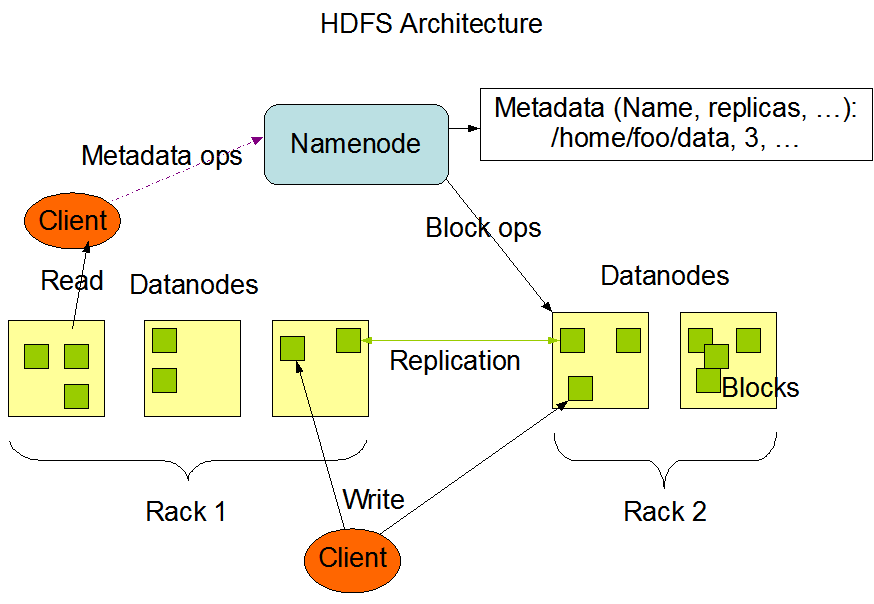
\includegraphics{img/hdfsarchitecture.png}
\caption{Schema di funzionamento dell'architettura di HDFS}
\end{figure}

La documentazione di Hadoop descrive i seguenti come i principi
architetturali alla base della progettazione di HDFS:

\begin{itemize}
\item
  \textbf{Fallimento hardware come regola invece che come eccezione}

  Un sistema che esegue HDFS è composto da molti componenti, con
  probabilità di fallimento non triviale. Sulla base di questo
  principio, HDFS da' per scontato che \textbf{ci sia sempre un numero
  di componenti non funzionanti}, e si pone di rilevare errori e guasti
  e di fornire un recupero rapido e automatico da questi.

  Il meccanismo principale con cui HDFS raggiunge questo obiettivo è la
  replicazione: in un cluster, ogni blocco di cui un file è composto è
  replicato in più macchine (3 di default). Se un blocco non è
  disponibile in una macchina, o se non supera i controlli di integrità,
  una sua copia può essere letta da un'altra macchina in modo
  trasparente per il client.

  Il numero di repliche per ogni blocco è configurabile, e ci sono più
  criteri con cui viene deciso in quali macchine il blocco viene
  replicato, principalmente orientati al risparmio di banda di rete.
\item
  \textbf{Modello di coerenza semplice}

  Per semplificare l'architettura generale, HDFS fa delle assunzioni
  specifiche sul tipo di dati che vengono salvati in HDFS e pone dei
  limiti su come l'utente possa lavorare sui file. In particolare,
  \textbf{non è possibile modificare arbitrariamente file già
  esistenti}, e le modifiche devono limitarsi a operazioni di
  troncamento e di aggiunta a fine file. Queste supposizioni permettono
  di semplificare il modello di coerenza, perché i blocchi di dati, una
  volta scritti, possono essere considerati immutabili, evitando una
  considerevole quantità di problemi in un ambiente dove i blocchi di
  dati sono replicati in più posti:

  \begin{itemize}
  \item
    Per ogni modifica a un blocco di dati, bisognerebbe verificare quali
    altre macchine contengono il blocco, e rieseguire la modifica (o
    rireplicare il blocco modificato) in ognuna di queste.
  \item
    Queste modifiche dovrebbero essere fatte in modo atomico, o
    richieste di lettura su una determinata replica di un blocco invece
    che in un'altra potrebbe portare a risultati inconsistenti o non
    aggiornati.
  \end{itemize}

  Le limitazioni che Hadoop impone sono ragionevoli per lo use-case per
  cui HDFS è progettato, caratterizzato da grandi dataset che vengono
  copiati nel filesystem e letti in blocco.
\item
  \textbf{Dataset di grandi dimensioni}

  I filesystem distribuiti sono generalmente necessari per aumentare la
  capacità di storage disponibile oltre quella di una singola macchina.
  La distribuzione di HDFS, assieme alla grande dimensione dei blocchi
\item
  \textbf{Accesso in streaming}

  HDFS predilige l'accesso ai dati in streaming, per permettere ai
  lavori batch di essere eseguiti con grande efficienza. Questo
  approccio va a discapito del tempo di latenza della lettura dei file,
  ma permette di avere un throughput in lettura molto vicino ai tempi di
  lettura del disco.
\item
  \textbf{Portabilità su piattaforme software e hardware eterogenee}

  HDFS è scritto in Java, ed è portabile in tutti i sistemi che ne
  supportano il runtime.
\end{itemize}

L'architettura di HDFS è di tipo master/slave, dove un nodo centrale,
chiamato \textbf{NameNode}, gestisce i metadati e la struttura del
filesystem, mentre i nodi slave, chiamati \textbf{DataNode}, contengono
i blocchi di cui file sono composti. Tipicamente, viene eseguita
un'istanza del software del DataNode per macchina del cluster, e una
macchina dedicata esegue il NameNode.

I \emph{client} del filesystem interagiscono sia con il NameNode che con
i DataNode per l'accesso ai file. La comunicazione tra il client e i
nodi avviene tramite socket TCP ed è coordinata dal NameNode, che
fornisce ai client tutte le informazioni sul filesystem e su quali nodi
contengono i DataBlock dei file richiesti.

\subsection{Comunicare con HDFS}\label{comunicare-con-hdfs}

Hadoop fornisce tool e librerie che possono agire da client nei
confronti di HDFS. Il tool più diretto è la CLI, accessibile nelle
macchine in cui è installato Hadoop tramite il comando
\texttt{hadoop\ fs}.

\begin{Shaded}
\begin{Highlighting}[]
\ExtensionTok{%}\NormalTok{ hadoop fs -help}
\ExtensionTok{Usage}\NormalTok{: hadoop fs [generic options]}
\NormalTok{    [}\ExtensionTok{-appendToFile} \OperatorTok{<}\NormalTok{localsrc}\OperatorTok{>}\NormalTok{ ... }\OperatorTok{<}\NormalTok{dst}\OperatorTok{>}\NormalTok{]}
\NormalTok{    [}\ExtensionTok{-cat}\NormalTok{ [-ignoreCrc] }\OperatorTok{<}\NormalTok{src}\OperatorTok{>}\NormalTok{ ...]}
\NormalTok{    [}\ExtensionTok{-checksum} \OperatorTok{<}\NormalTok{src}\OperatorTok{>}\NormalTok{ ...]}
\NormalTok{    [}\ExtensionTok{-chgrp}\NormalTok{ [-R] GROUP PATH...]}
\NormalTok{    [}\ExtensionTok{-chmod}\NormalTok{ [-R] }\OperatorTok{<}\NormalTok{MODE[,MODE]... }\KeywordTok{|} \ExtensionTok{OCTALMODE}\OperatorTok{>}\NormalTok{ PATH...]}
\NormalTok{    [}\ExtensionTok{-chown}\NormalTok{ [-R] [OWNER][:[GROUP]] PATH...]}
\NormalTok{    [}\ExtensionTok{-copyFromLocal}\NormalTok{ [-f] [-p] [-l] [-d] }\OperatorTok{<}\NormalTok{localsrc}\OperatorTok{>}\NormalTok{ ... }\OperatorTok{<}\NormalTok{dst}\OperatorTok{>}\NormalTok{]}
\NormalTok{    [}\ExtensionTok{-copyToLocal}\NormalTok{ [-f] [-p] [-ignoreCrc] [-crc] }\OperatorTok{<}\NormalTok{src}\OperatorTok{>}\NormalTok{ ... }\OperatorTok{<}\NormalTok{localdst}\OperatorTok{>}\NormalTok{]}
\NormalTok{    [}\ExtensionTok{-count}\NormalTok{ [-q] [-h] [-v] [-t [}\OperatorTok{<}\NormalTok{storage type}\OperatorTok{>}\NormalTok{]] [-u] [-x] }\OperatorTok{<}\NormalTok{path}\OperatorTok{>}\NormalTok{ ...]}
\NormalTok{    [}\ExtensionTok{-cp}\NormalTok{ [-f] [-p }\KeywordTok{|} \ExtensionTok{-p}\NormalTok{[topax]] [-d] }\OperatorTok{<}\NormalTok{src}\OperatorTok{>}\NormalTok{ ... }\OperatorTok{<}\NormalTok{dst}\OperatorTok{>}\NormalTok{]}
\ExtensionTok{...}
\end{Highlighting}
\end{Shaded}

La CLI fornisce alcuni comandi comuni nei sistemi POSIX, come
\texttt{cp}, \texttt{rm}, \texttt{mv}, \texttt{ls} e \texttt{chown}, e
altri che riguardano specificamente HDFS, come \texttt{copyFromLocal} e
\texttt{copyToLocal}, utili a trasferire dati tra la macchina su cui si
opera e il filesystem.

I comandi richiedono l'URI che identifica l'entità su cui si vuole
operare. Per riferirsi a una risorsa all'interno di un'istanza di HDFS,
si usa l'URI del namenode, con schema \texttt{hdfs}\footnote{Hadoop è
  abbastanza generale da poter lavorare con diversi filesystem, con lo
  schema definisce il protocollo di comunicazione, che non deve essere
  necessariamente \texttt{hdfs}. Ad esempio, un URI con schema
  \texttt{file} si riferisce al filesystem locale, e le operazioni
  eseguite su URI che utilizzano questo schema vengono effettuate sulla
  macchina dove viene eseguito il comando. Questo approccio può essere
  adatto nella fase di testing dei programmi, ma nella maggior parte dei
  casi è comunque desiderabile lavorare su un filesystem distribuito
  adeguato alla gestione dei Big Data, e un'alternativa ad HDFS degna di
  nota è MapR-FS{[}\protect\hyperlink{ref-mapr-fs}{8}{]}.}, e con il
path corrispondente al percorso della risorsa nel filesystem. Ad
esempio, è possibile creare una cartella \texttt{foo} all'interno della
radice del filesystem con il seguente comando:

\begin{Shaded}
\begin{Highlighting}[]
\ExtensionTok{hadoop}\NormalTok{ fs -mkdir hdfs://localhost:8020/foo}
\end{Highlighting}
\end{Shaded}

Per diminuire la verbosità dei comandi è possibile utilizzare percorsi
relativi, e specificare l'opzione \texttt{dfs.defaultFS} nella
configurazione di Hadoop all'URI del filesystem ai cui i percorsi
relativi si riferiscono. In questo modo, si può accorciare l'esempio
precedente a:

\begin{Shaded}
\begin{Highlighting}[]
\ExtensionTok{hadoop}\NormalTok{ fs -mkdir foo}
\end{Highlighting}
\end{Shaded}

Ad esempio, data la seguente cartella:

\begin{Shaded}
\begin{Highlighting}[]
\NormalTok{[}\ExtensionTok{root@sandbox}\NormalTok{ example_data]# ls}
\ExtensionTok{example1.txt}\NormalTok{  example2.txt  example3.txt}
\end{Highlighting}
\end{Shaded}

Si possono copiare i file dalla cartella locale della macchina al
filesystem distribuito con il seguente comando:

\begin{Shaded}
\begin{Highlighting}[]
\NormalTok{[}\ExtensionTok{root@sandbox}\NormalTok{ example_data]# hadoop fs -copyFromLocal example*.txt /example}
\end{Highlighting}
\end{Shaded}

Per verificare che l'operazione sia andata a buon fine, si può ottenere
un listing della cartella in cui si sono trasferiti i file con il
comando \texttt{ls}:

\begin{Shaded}
\begin{Highlighting}[]
\NormalTok{[}\ExtensionTok{root@sandbox}\NormalTok{ example_data]# hadoop fs -ls /example}
\ExtensionTok{Found}\NormalTok{ 3 items}
\ExtensionTok{-rw-r--r--}\NormalTok{   1 root hdfs         70 2017-06-30 03:58 /example/example1.txt}
\ExtensionTok{-rw-r--r--}\NormalTok{   1 root hdfs         39 2017-06-30 03:58 /example/example2.txt}
\ExtensionTok{-rw-r--r--}\NormalTok{   1 root hdfs         43 2017-06-30 03:58 /example/example3.txt}
\end{Highlighting}
\end{Shaded}

Il listing è molto simile a quello ottenibile su sistemi Unix. Una
differenza importante è la seconda colonna, che non mostra il numero di
hard link al file nel filesystem\footnote{HDFS correntemente non
  supporta link nel filesystem.}, ma il numero di repliche che HDFS ha a
disposizione del file, in questo caso una per file. Il numero di
repliche fatte da HDFS può essere impostato settando il fattore di
replicazione di default, che per Hadoop in modalità distribuita è 3 di
default. Si può anche cambiare il numero di repliche disponibili per
determinati file, utilizzando il comando \texttt{hdfs\ dfs}:

\begin{Shaded}
\begin{Highlighting}[]
\NormalTok{[}\ExtensionTok{root@sandbox}\NormalTok{ ~]# hdfs dfs -setrep 2 /example/example1.txt}
\ExtensionTok{Replication}\NormalTok{ 2 set: /example/example1.txt}
\NormalTok{[}\ExtensionTok{root@sandbox}\NormalTok{ ~]# hadoop fs -ls /example}
\ExtensionTok{Found}\NormalTok{ 3 items}
\ExtensionTok{-rw-r--r--}\NormalTok{   2 root hdfs         70 2017-06-30 03:58 /example/example1.txt}
\ExtensionTok{-rw-r--r--}\NormalTok{   1 root hdfs         39 2017-06-30 03:58 /example/example2.txt}
\ExtensionTok{-rw-r--r--}\NormalTok{   1 root hdfs         43 2017-06-30 03:58 /example/example3.txt}
\end{Highlighting}
\end{Shaded}

HDFS è anche accessibile tramite \emph{HDFS Web Interface}, un tool che
fornisce informazioni sullo stato generale del filesystem e sul suo
contenuto. Ci sono anche tool di amministrazione di cluster Hadoop che
offrono GUI web più avanzate di quella fornita di default da HDFS. Due
esempi sono Cloudera Manager e Apache Ambari, che offrono un file
manager lato web con cui è possibile interagire in modo più semplice,
permettendo anche a utenti in ambito meno tecnico di lavorare con il
filesystem.

\begin{figure}
\centering
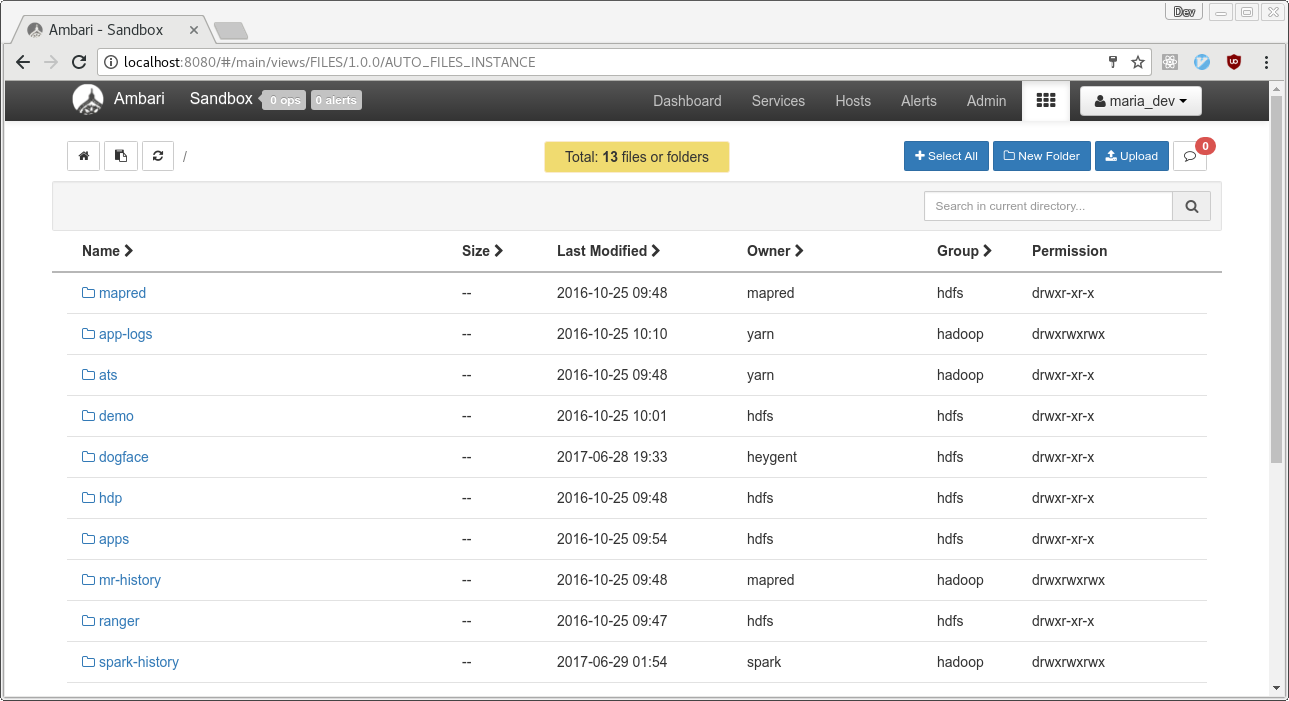
\includegraphics{img/ambari_hdfs.png}
\caption{Screenshot del file manager HDFS incluso in Ambari}
\end{figure}

Un'altra interfaccia importante ad HDFS è l'API \texttt{FileSystem} di
Hadoop, che permette un accesso programmatico da linguaggi per JVM a
tutte le funzioni del filesystem. L'API è generale, in modo che possa
essere utilizzata con filesystem diversi da HDFS.

Per linguaggi che non supportano interfacce Java, esiste
un'implementazione in C chiamata \texttt{libhdfs}, che si appoggia sulla
Java Native Interface per esporre l'API di Hadoop.

Esistono poi progetti che permettono il montaggio di HDFS in un
filesystem locale. Alcune di queste implementazioni sono basate su FUSE,
mentre altre su NFS Gateway. Questo metodo di accesso permette
l'utilizzo di utilità native del sistema in uso in HDFS.

\subsection{NameNode}\label{namenode}

Il NameNode è il riferimento centrale per i metadati del filesystem nel
cluster, il che vuol dire che se il NameNode non è disponibile il
filesystem non è accessibile. Questo rende il NameNode un \emph{single
point of failure} del sistema, e per questa ragione HDFS mette a
disposizione dei meccanismi per attenutare l'indisponibilità del sistema
in caso di non reperibilità del NameNode, e per assicurare che lo stato
del filesystem possa essere recuperato a partire dal NameNode.

Il NameNode è anche il nodo a cui i client si connettono alla lettura
del file. La connessione ha il solo scopo di fornire le informazioni sui
DataNode che contengono i dati effettivi del file. I dati di un file non
passano mai per il NameNode.

Tuttavia, il NameNode non salva persistentemente le informazioni sulle
posizioni dei blocchi, che vengono invece mantenute dai DataNode. Perché
il NameNode possa avere in memoria le informazioni sui file necessarie
per essere operativo, questo deve ricevere le liste dei blocchi in
possesso dei DataNode, in messaggi chiamati \textbf{block report}. Non è
necessario che il DataNode conosca la posizione di tutti i blocchi sin
dall'inizio, ma basta che per ogni blocco conosca la posizione di un
numero minimo di repliche, determinato da un'opzione chiamata
\texttt{dfs.replication.min.replicas}, di default 1.

Questa procedura avviene quando il NameNode si trova in uno stato
chiamato \textbf{safe mode}.

\subsubsection{\texorpdfstring{\emph{Namespace image} ed \emph{edit
log}}{Namespace image ed edit log}}\label{namespace-image-ed-edit-log}

Le informazioni sui metadati del sistema vengono salvate nello storage
del NameNode in due posti, la \emph{\textbf{namespace image}} e
l'\emph{\textbf{edit log}}. La \emph{namespace image} è uno snapshot
dell'intera struttura del filesystem, mentre l'\emph{edit log} è un
elenco di operazioni eseguite nel filesystem a partire dalla
\emph{namespace image}. Partendo dalla \emph{namespace image} e
applicando le operazioni registrate nell'\emph{edit log}, è possibile
risalire allo stato attuale del filesystem. Il NameNode ha una
rappresentazione dello stato del filesystem anche nella memoria
centrale, che viene utilizzata per servire le richieste di lettura.

Quando HDFS riceve una richiesta che richiede la modifica dei metadati,
il NameNode esegue le seguenti operazioni:

\begin{enumerate}
\tightlist
\item
  registra la transazione nell'\emph{edit log}
\item
  aggiorna la rappresentazione del filesystem in memoria
\item
  passa all'operazione successiva.
\end{enumerate}

La ragione per cui i cambiamenti dei metadati vengono registrati
nell'\emph{edit log} invece che nella \emph{namespace image} è la
velocità di scrittura: scrivere ogni cambiamento del filesystem mano a
mano che avviene nell'immagine sarebbe lento, dato che questa può avere
dimensioni nell'ordine dei gigabyte. Il NameNode esegue un \emph{merge}
dell'\emph{edit log} e della \emph{namespace image} a ogni suo avvio,
portando lo stato attuale dell'immagine al pari di quello del
filesystem.

Dato che la dimensione dell'\emph{edit log} può diventare notevole, è
utile eseguire l'operazione di \emph{merge} al raggiungimento di una
soglia di dimensione del log. Questa operazione è computazionalmente
costosa, e se fosse eseguita dal NameNode potrebbe interferire con la
sua operazione di routine.

Per evitare interruzioni nel NameNode, il compito di eseguire
periodicamente il \emph{merge} dell'\emph{edit log} è affidato a
un'altra entità, il \textbf{Secondary NameNode}. Il Secondary NameNode
viene solitamente eseguito su una macchina differente, dato che richiede
un'unità di elaborazione potente e almeno la stessa memoria del NameNode
per eseguire l'operazione di merge.

\subsubsection{\texorpdfstring{Avvio del NameNode e \emph{Safe
Mode}}{Avvio del NameNode e Safe Mode}}\label{avvio-del-namenode-e-safe-mode}

Prima di essere operativo, il NameNode deve eseguire alcune operazioni
di startup, tra cui attendere di aver ricevuto i block report dai
DataNode in modo da conoscere le posizioni dei blocchi. Durante queste
operazioni, il NameNode si trova in uno stato chiamato \emph{safe mode},
in cui sono permesse unicamente operazioni che accedono ai metadati del
filesystem, e tentativi di lettura e scrittura di file falliscono. Prima
di poter permettere l'accesso completo, il NameNode ha bisogno di
ricevere le informazioni sui blocchi da parte dei DataNode.

Per ricapitolare, al suo avvio, il NameNode effettua il merge della
\emph{namespace image} con l'\emph{edit log}. Al termine
dell'operazione, il risultato del merge viene salvato come la nuova
\emph{namespace image}. Il Secondary NameNode non viene coinvolto in
questo primo merge.

Prima di uscire dalla safe mode, il NameNode attende di avere abbastanza
informazioni da poter accedere a un numero minimo di repliche di ogni
blocco. A questo punto il NameNode esce dalla safe mode.

Si possono utilizzare dei comandi per verificare lo stato, attivare e
disattivare la safe mode.

\begin{Shaded}
\begin{Highlighting}[]
\ExtensionTok{bash-4.1}\NormalTok{$ hdfs dfsadmin -safemode get}
\ExtensionTok{Safe}\NormalTok{ mode is OFF}
\ExtensionTok{bash-4.1}\NormalTok{$ hdfs dfsadmin -safemode enter}
\ExtensionTok{Safe}\NormalTok{ mode is ON}
\ExtensionTok{bash-4.1}\NormalTok{$ hdfs dfsadmin -safemode leave}
\ExtensionTok{Safe}\NormalTok{ mode is OFF}
\end{Highlighting}
\end{Shaded}

\begin{figure}
\centering
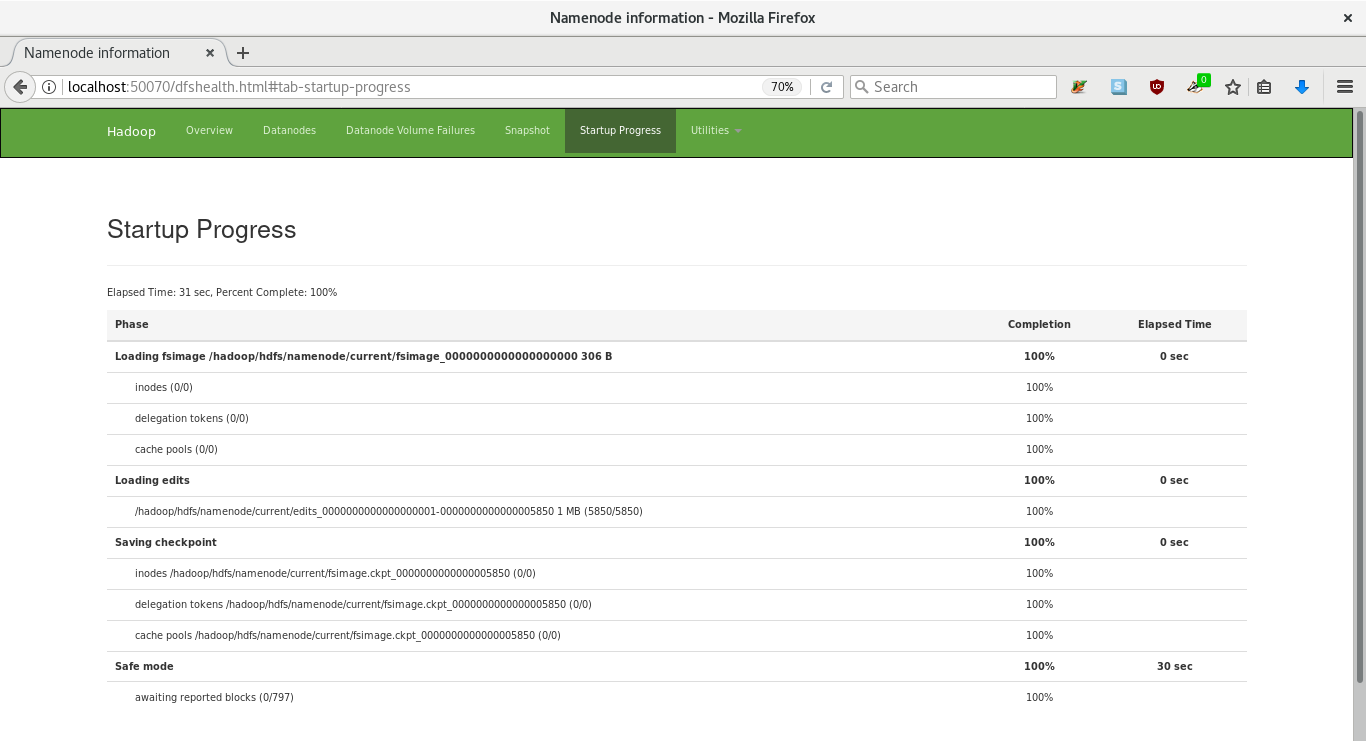
\includegraphics{img/hdfs-web-startup.png}
\caption{Lo stato dello startup di un'istanza di HDFS, mostrata da HDFS
Web Interface.}
\end{figure}

\subsection{Processo di lettura di file in
HDFS}\label{processo-di-lettura-di-file-in-hdfs}

\begin{figure}
\centering
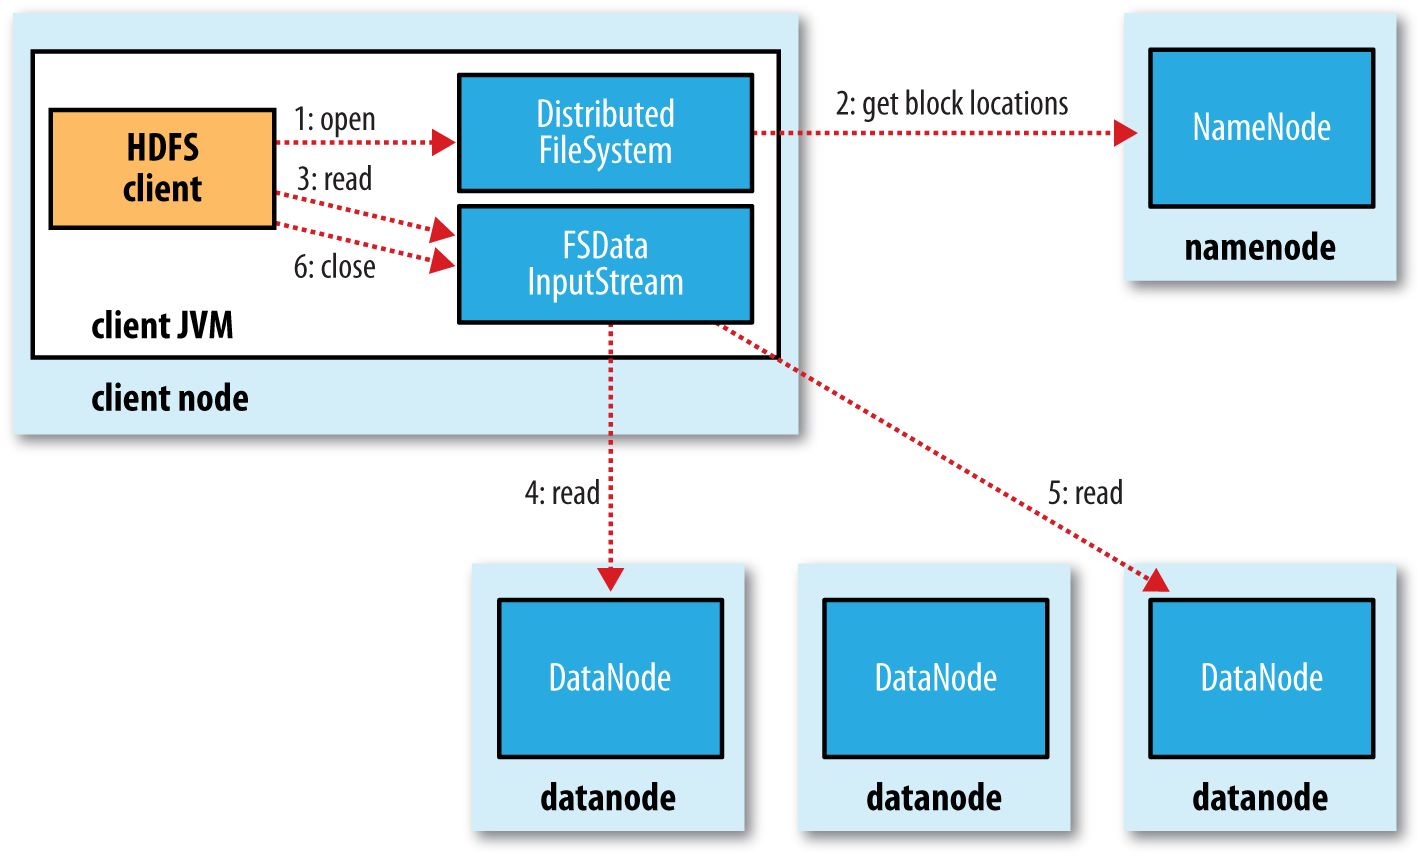
\includegraphics{img/hdfs-file-read.png}
\caption{Diagramma delle operazioni eseguite nella lettura di un file in
HDFS{[}\protect\hyperlink{ref-hadoop-guide-hdfs-file-read}{1}{]}}
\end{figure}

Per avere un quadro completo del funzionamento di HDFS, è utile
osservare come avvenga il processo di lettura di un file. In questa
sezione si prende in esame un programma di esempio che utilizza le API
di HDFS per reimplementare una versione semplificata del comando
\texttt{cat}, confrontano le interfacce Java utilizzate con le
operazioni a cui queste corrispondono.

\begin{codelisting}

\caption{Programma di esempio che reimplementa il comando \texttt{cat}.}

\hypertarget{lst:hdfs-cat}{\label{lst:hdfs-cat}}
\begin{Shaded}
\begin{Highlighting}[numbers=left,,]
\KeywordTok{import}\ImportTok{ java.io.InputStream;}
\KeywordTok{import}\ImportTok{ java.net.URI;}

\KeywordTok{import}\ImportTok{ org.apache.hadoop.conf.Configuration;}
\KeywordTok{import}\ImportTok{ org.apache.hadoop.fs.FileSystem;}
\KeywordTok{import}\ImportTok{ org.apache.hadoop.fs.Path;}
\KeywordTok{import}\ImportTok{ org.apache.hadoop.io.IOUtils;}

\KeywordTok{public} \KeywordTok{class}\NormalTok{ MyCat \{}

    \KeywordTok{public} \DataTypeTok{static} \DataTypeTok{void} \FunctionTok{main}\NormalTok{(}\BuiltInTok{String}\NormalTok{ args[]) }\KeywordTok{throws} \BuiltInTok{Exception}\NormalTok{ \{}

        \BuiltInTok{String}\NormalTok{ source = args[}\DecValTok{0}\NormalTok{];}
        \BuiltInTok{Configuration}\NormalTok{ conf = }\KeywordTok{new} \BuiltInTok{Configuration}\NormalTok{();}

\NormalTok{        FileSystem sourcefs = FileSystem.}\FunctionTok{get}\NormalTok{(}\BuiltInTok{URI}\NormalTok{.}\FunctionTok{create}\NormalTok{(source), conf);}

        \BuiltInTok{InputStream}\NormalTok{ in = }\KeywordTok{null}\NormalTok{;}

        \KeywordTok{try}\NormalTok{ \{}
\NormalTok{            in = sourcefs.}\FunctionTok{open}\NormalTok{(}\KeywordTok{new} \FunctionTok{Path}\NormalTok{(source));}
\NormalTok{            IOUtils.}\FunctionTok{copyBytes}\NormalTok{(in, }\BuiltInTok{System}\NormalTok{.}\FunctionTok{out}\NormalTok{, }\DecValTok{4096}\NormalTok{, }\KeywordTok{false}\NormalTok{);}
\NormalTok{        \} }\KeywordTok{finally}\NormalTok{ \{}
\NormalTok{            IOUtils.}\FunctionTok{closeStream}\NormalTok{(in);}
\NormalTok{        \}}
\NormalTok{    \}}
\NormalTok{\}}
\end{Highlighting}
\end{Shaded}

\end{codelisting}

I passi che vengono eseguiti nel programma sono i seguenti:

\begin{enumerate}
\tightlist
\item
  Creare un oggetto \texttt{org.apache.hadoop.conf.Configuration}. Gli
  oggetti \texttt{Configuration} contengono le impostazioni
\end{enumerate}

\section{MapReduce}\label{mapreduce}

Per dare un'idea concreta di come funziona la programmazione in un
cluster Hadoop

MapReduce è il primo importante modello di programmazione a cui Hadoop
fa riferimento per l'esecuzione di applicazioni distribuite. Hadoop è
stato scritto e pensato per l'esecuzione di lavori MapReduce, e nelle
prime versioni era il solo modello di programmazione disponibile.

I lavori MapReduce

\chapter{Spark}\label{spark}

Apache Spark è un framework per il batch processing, che è in grado di a

\chapter{Strumenti per lo Stream
Processing}\label{strumenti-per-lo-stream-processing}

\chapter{NoSQL e Big Data}\label{nosql-e-big-data}

\chapter*{Bibliografia}\label{bibliografia}
\addcontentsline{toc}{chapter}{Bibliografia}

\hypertarget{refs}{}
\hypertarget{ref-hadoop-guide-hdfs-file-read}{}
1. White T (2015) Hadoop: The Definitive Guide. 69.

\hypertarget{ref-hadoop-adoption-survey}{}
2. Gartner Survey Highlights Challenges to Hadoop Adoption. In: Gartner.
\url{http://www.gartner.com/newsroom/id/3051717}.

\hypertarget{ref-hadoop-market-analysis}{}
3. Hadoop Market Forecast 2017-2022. In: Market Analysis.
\url{https://www.marketanalysis.com/?p=279}.

\hypertarget{ref-digital-univ}{}
4. The Digital Universe of Opportunities: Rich Data and the Increasing
Value of the Internet of Things.

\hypertarget{ref-hadoop-doc-main}{}
5. Apache Hadoop Documentation. \url{https://hadoop.apache.org/}.

\hypertarget{ref-hadoop-ppa}{}
6. Hadoop Ubuntu Packagers PPA.
\url{https://launchpad.net/~hadoop-ubuntu/+archive/ubuntu/stable}.

\hypertarget{ref-hadoop-aur}{}
7. AUR - Hadoop. \url{https://aur.archlinux.org/packages/hadoop/}.

\hypertarget{ref-mapr-fs}{}
8. MapR-FS Overview. \url{https://mapr.com/products/mapr-fs/}.

\end{document}
